\chapter{Aho-Corasick} \label{chap:aho}

Neste capítulo vamos apresentar um algoritmo que recebe um conjunto de strings~${\cS = \{S_1, \ldots, S_k\}}$ de tamanho~$n$ e uma string~$P$, e determina, para cada~$S_i \in \cS$, quais são suas ocorrências em~$P$.
Seja~$T$ uma trie para o conjunto~$\cS$ e~$r$ sua raiz.

Com~$T$, é possível descobrir quais strings de~$\cS$ são prefixos de~$P$ em tempo~$\Oh(|P|)$. Com isso é possível encontrar todas as ocorrências de strings de~$\cS$ em~$P$ em tempo~$\Oh(|P|^2)$, usando esse mesmo algoritmo para todos os sufixos de~$P$.

O algoritmo apresentado nesse capítulo é conhecido como Aho-Corasick e foi criado por Alfred V. Aho and Margaret J. Corasick \cite{aho}. Com preprocessamento de~$T$ que consome tempo~$\Oh(n|\E|)$, similar ao preprocessamento do algoritmo KMP, conseguimos com esse algoritmo buscar todas as ocorrências das strings de~$\cS$ em~$P$ em tempo~$\Oh(|P| + x)$, onde~$x$ é o número de ocorrências de strings de~$\cS$ em~$P$.

\section{Link de falha}

Para cada nó~$v$ de~$T$, defina~$S(v)$ como a string associada a~$v$ em~$T$, e~$d(v) \coloneqq |S(v)|$ sua profundidade. Para cada nó~$v \neq r$, seja~$f(v)$ o nó~$u$ com maior~$d(u)$ tal que~$S(u) \suffp S(v)$. Ou seja, o nó de maior profundidade cuja string associada é sufixo próprio de~$S(v)$.

Note que a string vazia associada à raiz é um sufixo próprio de todas outras strings, assim~$f(v)$ existe para todo~$v \neq r$. O valor~$f(v)$ é chamado de \emph{link de falha} de~$v$.

A Figura~\ref{fig:triefail} mostra a trie da Figura~\ref{fig:triesimple} com todos os links de falha que não apontam para a raiz desenhados. Note que um link de falha não necessariamente aponta para um ancestral do nó.

\begin{figure}
\centering
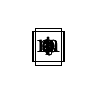
\begin{tikzpicture}[sibling distance=30pt]
\Tree [.{}
[.\node(m){m}; [.\node(ma){a}; [.\node(mam){m}; [.\node(mama){a}; [.\node(mamat){t}; \node[draw](mamata){a}; ] ] ] [.\node(mat){t}; \node[draw](mata){a}; ] ] ]
[.\node(o){o}; [.\node[draw](oi){i}; [.\node(oit){t}; \node[draw](oito){o}; ] ] [.\node(om){m}; [.\node(oma){a}; \node[draw](omar){r}; ] ] ]
]
%\draw[semithick,->] (t)..controls +(south west:5) and +(south:5)..(wh);
\draw[densely dotted,->] (mamata) -- (mata);
\draw[densely dotted,->] (mamat) -- (mat);
\draw[densely dotted,->] (mama) -- (ma);
\draw[densely dotted,->] (mam) -- (m);
\draw[densely dotted,->] (oito) -- (o);
\draw[densely dotted,->] (oma) -- (ma);
\draw[densely dotted,->] (om) -- (m);
\end{tikzpicture}
\caption{Trie~$T$ com links de falha.} \label{fig:triefail}
\end{figure}

O seguinte algoritmo calcula corretamente o valor de~$f(v)$, se~$v$ não é filho da raiz. Seja~$c(v)$ o caractere associado à aresta que entra em~$v$ e~$p(v)$ o pai de~$v$ em~$T$. Também assuma que~$v(c)$ é o filho de~$v$ por uma aresta de caractere~$c$, ou \keyword{null} se esta não existir. Se~$v$ é filho da raiz, então~$f(v) = r$.

\begin{algorithm} [ht]
\begin{algorithmic}[1]
\Function {AuxiliaryLinks}{$v$}
    \State $f(v) = f(p(v))$
    \While {$f(v) \neq r \And f(v)(c(v)) = \Null$}
        \State $f(v) = f(f(v))$
    \EndWhile
    \If {$f(v)(c(v)) \neq \Null$}
        \State $f(v) = f(v)(c(v))$
    \EndIf
    \algstore{auxiliarylinks}
\end{algorithmic}
\end{algorithm}

Note que \func{AuxiliaryLinks}{v} precisa que os valores de~$f$ já estejam calculados para o pai de~$v$, e todos os outros vértices com profundidade menor que a do pai de~$v$. É possível conseguir isso se calcularmos os valores de~$f$ na mesma ordem que descobrirmos os vértices usando uma busca em largura (BFS) a partir da raiz. Quando estamos analisando um nó, todos com distância menor já foram analisados.

\section{Link de ocorrência}
\label{sec:linkoc}

Para descobrir as ocorrências das strings de~$\cS$ em~$P$, devemos processar um a um cada caractere de~$P$. Após analisar o caractere~$P[i]$, estaremos no nó~$v_i$ tal que~$S(v_i)$ é o maior prefixo de alguma string de~$\cS$ que é sufixo de~$P[1\tdots i]$. Se para algum~$i$ temos que~$v_i$ está marcado em~$T$, então temos uma ocorrência da string~$S(v_i)$ que acaba na posição~$i$ de~$P$. Mas essa não é a única situação em que temos ocorrências.

Se algum sufixo próprio de~$S(v_i)$ for uma string em~$\cS$, então essa string também ocorre em~$P$ acabando na posição~$i$, mesmo que o nó~$v_i$ não seja um nó marcado. Por exemplo, na trie da Figura~\ref{fig:triefail}, para o texto~$P = \texttt{amamatax}$,~$S(v_7) = \texttt{mamata}$, mas além da ocorrência dessa string, também existe a ocorrência de \texttt{mata} na mesma posição.

Para verificar esse tipo de ocorrência, para cada nó~$v$ de~$T$, defina~$N(v)$, o chamado \emph{link de ocorrência}, como o nó~$u$ com~$d(u)$ máximo tal que~$S(u) \suffp S(v)$ e~$u$ está marcado, ou \keyword{null} se tal nó não existe. Ou seja,~$N(v)$ é o primeiro vértice atingível ``caminhando'' pelos links de falha que é um nó marcado. Assim se, ao analisar~$P[i]$, estamos no nó~$v_i$ e~$N(v_i) \neq \text{\keyword{null}}$, então uma ocorrência de~$S(N(v_i))$ termina na posição~$i$ de~$P$.

Dessa forma, ``caminhando'' pelos links de ocorrência de~$v_i$, conseguimos determinar todas as strings de~$\cS$ que têm uma ocorrência em~$P$ terminando na posição~$i$, em tempo proporcional ao número de tais ocorrências (pois cada link de ocorrência leva para uma ocorrência e leva tempo~$\Oh(1)$ para ser percorrido).

Calcular esses links é fácil. Basta adicionar ao final da rotina \func{AuxiliaryLinks}{v}

\begin{algorithm}[ht]
\begin{algorithmic}[1]
    \algrestore{auxiliarylinks}
    \If {$f(v).mrk = \True$}
        \State $N(v) = f(v)$
    \Else
        \State $N(v) = N(f(v))$
    \EndIf
\EndFunction
\end{algorithmic}
\end{algorithm}

\section{Preprocessamento dos links auxiliares}
\label{sec:ahopre}

A construção dos links de falha e de ocorrência pode ser feita da seguinte forma, dado que a trie para~$\cS$ já está construída.

\begin{algorithm}
\caption{Preprocessamento do algoritmo de Aho-Corasick}\label{lst:ahopre}
\begin{algorithmic}[1]
\State $Q = \{\}$ \Comment {fila vazia}
\For{$c \in \E$}
    \If {$r(c) \neq \Null$}
        \State $Q.push(r(c))$
        \State $f(r(c)) = r$
        \State $N(r(c)) = \Null$
    \EndIf
\EndFor
\While {$Q \neq \{\}$}
    \State $u = Q.pop()$
    \For {$c \in \E$}
        \If {$u(c) \neq \Null$}
            \State \func{AuxiliaryLinks}{u(c)}
            \State $Q.push(u(c))$
        \EndIf
    \EndFor
\EndWhile
\end{algorithmic}
\end{algorithm}

\begin{theorem}
O algoritmo apresentado no Código~\ref{lst:ahopre} calcula corretamente~$f$ e~$N$ para todo nó~$v$ da trie~$T$ cuja raiz é~$r$.
\end{theorem}

\begin{proof}
Seja~$T$ a trie. O algoritmo realiza uma BFS nos nós de~$T$, e aciona \func{AuxiliaryLinks}{v} do nó~$v$ no momento em que adiciona v à fila da BFS. Nesse momento, os links do pai de~$v$ e de todos vértices com distância à raiz menor já foram calculados.

Vamos usar que, se~$S$ é uma string, então~$\pop(S) := S[1\tdots |S|-1]$, ou seja, a string~$S$ removendo-se seu último caractere.

Vamos provar inicialmente que~$f$ é calculado corretamente. Como~${\pop(S(v)) = S(u)}$, onde~$u$ é o pai de~$v$, temos que~$\pop(S(f(v))) \suff S(f(u)) \suffp S(u)$, ou seja, para encontrar~$f(v)$, devemos encontrar o maior sufixo próprio de~$S(u)$ cujo nó tem um filho com aresta associada a~$c(v)$.

Queremos então mostrar que o \keyword{while} nas linhas 3-4 de \func{AuxiliaryLinks}{v} itera por todos os sufixos próprios de~$S(u)$ que têm nós em~$T$, em ordem decrescente de tamanho. Se mostrarmos isso, então o algoritmo escolhe o maior deles que também satisfaz a restrição adicional, e portanto a resposta está correta. Note que se a resposta for a raiz, como~$d(v) > 1$, então não existe nenhum tal prefixo que satisfaça a segunda condição do~\keyword{while}, logo o algoritmo também funciona corretamente.

Observe que~$f(v)$ é inicializado com~$f(u)$. Como assumimos que este está calculado corretamente, ele é o maior sufixo próprio de~$S(u)$ em~$T$ pela definição de~$f$. Note que~${d(f(w)) < d(w)}$, para todo nó~$w$. Logo o~\keyword{while} está iterando em ordem decrescente de tamanho dos sufixos. Como~$f(w)$ é sempre o~\emph{maior} sufixo próprio de~$S(w)$, nenhum sufixo de~$S(u)$ vai deixar de ser visitado, logo o~\keyword{while} itera por todos sufixos de~$S(u)$ e calcula o valor de~$f(v)$ corretamente.

Para calcular~$N(v)$, devemos encontrar o primeiro nó entre~$f(v), f(f(v)), \ldots, r$ que é marcado. Se~$f(v)$ está marcado, então~$N(v) = f(v)$, caso contrário,~$N(f(v))$ é o primeiro nó marcado em~$f(f(v)), \ldots, r$, e então é o primeiro nó marcado em~$f(v), f(f(v)), \ldots, r$.

\end{proof}


\begin{complexity}
O algoritmo apresentado no Código~\ref{lst:ahopre} calcula os valores de~$f$ e~$N$ para todos os nós em tempo~$\Oh(n|\E|)$.
\end{complexity}

\begin{proof}
O laço da BFS claramente é executado uma vez para cada nó, e o laço interior é executado~$|\E|$ vezes. Logo o tempo é ~$\Omega(m|\E|)$, onde~$m$ é o número de vértices da trie, que é~$\Oh(n)$. Vamos mostrar que o cálculo dos valores de~$f$ e~$N$ levam no total tempo~$\Oh(n)$. Assim o tempo total fica~$\Oh(n|\E|)$.

O cálculo de~$N(v)$ claramente leva tempo~$\Oh(1)$ para cada nó da trie. Para~$S \in \cS$, sejam~$v_1, \ldots, v_{|S|}$ os nós associados a cada prefixo de~$S$ em~$T$. Seja~$w^S_i$ o número de iterações do \keyword{while} nas linhas 3-4 de \textsc{AuxiliaryLinks} para calcular~$f(v_i)$. Temos que~$0 \leq d(f(v_i)) < d(v_i)$ para todo~$i$, e~${d(f(v_{i+1})) \leq d(f(v_i)) + 1}$, pois o valor de~$f$ apenas ``avança'' no máximo uma vez por nó na linha 6 de \func{AuxiliaryLinks}{v}. Além, para cada iteração do \keyword{while},~$d(f(v_i))$ diminui de pelo menos~$1$, e para isso é necessário que tenha aumentado por essa quantidade em iterações anteriores. Então temos que~$\sum\limits_{i=2}^{|S_i|}{w^S_i} \leq |S|$.

Dessa forma~$\sum\limits_{i=1}^k{\sum\limits_{j=2}^{|S|}{w^{S_i}_j}} \leq \sum\limits_{i=1}^k{|S_i|} = n$, e o tempo total para calcular~$f$ é~$\Oh(n)$.
Logo o tempo total do preprocessamento é~$\Oh(n|\E|)$.
\end{proof}

\section{Busca}
\label{sec:ahobusca}

Como discutido no início da Seção~\ref{sec:linkoc}, para determinar as ocorrências de~$\cS$ em~$P$ devemos, após processar o caractere~$P[i]$, estar no nó~$v_i$ tal que~$S(v_i) \suff P[1\tdots i]$ e~$d(v_i)$ é máximo. Para isso usamos os links de falha, similarmente a como são usados no algoritmo~\func{AuxiliaryLinks}{v}. Ao processar~$P[i]$, queremos encontrar o maior sufixo de~$S(v_{i-1})$ que tem~$P[i]$ como próximo caractere (em alguma string de~$\cS$).
Para isso, basta usar os links de falha para iterar por todos esses sufixos.

\begin{algorithm}
\caption{Busca do algoritmo Aho-Corasick} \label{lst:ahobusca}
\begin{algorithmic}[1]
\State $u = r$
\For {$c \in P[1\tdots m]$}
    \While {$u \neq r \And u(c) = \Null$}
        \State $u = f(u)$
    \EndWhile
    \If {$u(c) \neq \Null$}
        \State $u = u(c)$
    \EndIf
    \If {$u.mrk = \True$}
        \State reportar ocorrência de~$u$
    \EndIf
    \State $x = u$
    \While{$N(x) \neq \Null$}
        \State $x = N(x)$
        \State reportar ocorrência de~$x$
    \EndWhile
\EndFor
\end{algorithmic}
\end{algorithm}

\subsection{Contagem de ocorrências}

O algoritmo apresentado no Código~\ref{lst:ahobusca} determina todas as ocorrências das strings de~$\cS$ em~$P$, e leva tempo~$\Oh(|P| + x)$, onde~$x$ é o número de tais ocorrências. Mas~$x$ é~$\Oh(|P|k)$, onde~$k$ é o número de strings em~$\cS$. Um caso ruim por exemplo é~$\cS = \{\text{a}, \text{aa}, \ldots\}$ e~${P = \text{aaa}\ldots\text{aa}}$, mas é claro que existem muitos outros casos menos óbvios em que~$x$ é~$\Theta(|P|k)$.

Por isso pode ser útil determinar apenas quais strings de~$\cS$ ocorrem no texto~$P$, ou ainda mais informação, como o número de ocorrências de cada string de~$\cS$ em~$P$. Adicionando um passo ao preprocessamento mostrado no Código~\ref{lst:ahopre} é possível desenvolver um algoritmo muito similar ao de busca que calcula o número de ocorrências de cada string de~$\cS$ em~$P$ em tempo~$\Oh(n + |P|)$, onde~$n$ é o tamanho de~$\cS$. Note que esse tempo independe do número de ocorrências.

Para cada nó~$v$ de~$T$ que não é a raiz, crie uma nova variável~$o(v)$, inicializada com~$0$, que ao final do algoritmo vai armazenar o número de ocorrências de~$S(v)$ em~$P$.

No Código~\ref{lst:ahobusca}, se substituirmos as linhas 7-12 pelo código abaixo, o cálculo dos valores~$o(v)$ é feito corretamente, pois na~$i$-ésima iteração~$v$ é o vértice com~$d(v)$ máximo tal que~$S(v) \suff P[1\tdots i]$, e dessa forma os vértices~$u$ de~$T$ tais que~$S(u) \suff P[1\tdots i]$ são todos os vértices atingíveis por~$v$ usando os links de falha.


\begin{algorithm}
\begin{algorithmic}[1]
\makeatletter
\setcounter{ALG@line}{4}
\makeatother
\Indent
    \State $\vdots$
    \State $x = u$
    \While {$x \neq r$}
        \State $o(x) \pluseq 1$
        \State $x = f(x)$
    \EndWhile
\EndIndent
\end{algorithmic}
\end{algorithm}


\begin{figure}
\centering
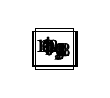
\begin{tikzpicture}[sibling distance=30pt]
\Tree [.\node(root){};
\edge[dotted]; [.\node(m){m$_1$}; \edge[dotted]; [.\node(ma){a$_1$}; \edge[dotted]; [.\node(mam){m$_2$}; \edge[dotted]; [.\node(mama){a$_2$}; \edge[dotted]; [.\node(mamat){t$_1$}; \edge[dotted]; \node[draw](mamata){a$_3$}; ] ] ] \edge[dotted]; [.\node(mat){t$_2$}; \edge[dotted]; \node[draw](mata){a$_4$}; ] ] ]
\edge[dotted]; [.\node(o){o$_1$}; \edge[dotted]; [.\node[draw](oi){i$_1$}; \edge[dotted]; [.\node(oit){t$_3$}; \edge[dotted]; \node[draw](oito){o$_2$}; ] ] \edge[dotted]; [.\node(om){m$_3$}; \edge[dotted]; [.\node(oma){a$_5$}; \edge[dotted]; \node[draw](omar){r$_1$}; ] ] ]
]
%\draw[semithick,->] (t)..controls +(south west:5) and +(south:5)..(wh);
\draw[->] (mamata) -- (mata);
\draw[->] (mamat) -- (mat);
\draw[->] (mama) -- (ma);
\draw[->] (mam) -- (m);
\draw[->] (oito) -- (o);
\draw[->] (oma) -- (ma);
\draw[->] (om) -- (m);
\end{tikzpicture}
\caption{Links de falha.} \label{fig:triefailonly}
\end{figure}

Observe que poderíamos, durante essa busca, apenas incrementar~$o(u)$, e depois de feita a busca, ``propagar'' todos esses valores ao mesmo tempo pelos links de falha. A Figura~\ref{fig:triefailonly} destaca os links de falha da trie da Figura~\ref{fig:triefail}, novamente sem mostrar os links para a raiz.

Considere um grafo~$T_f$ com os mesmos vértices da trie~$T$, mas onde as arestas são os links de falha de~$T$. Esse grafo é uma árvore, pois de cada nó exceto a raiz sai apenas um link de falha, e os links de falha sempre apontam para vértices com valor de~$d$ menor, logo não há ciclos. A Figura~\ref{fig:failtree} mostra como fica a árvore~$T_f$ do exemplo de trie da Figura~\ref{fig:triefailonly}.

\begin{figure}
\centering
\begin{tikzpicture}
\Tree [.{}
[.a$_1$ a$_2$ a$_5$ ]
[.a$_4$ a$_3$ ]
[.i$_1$ ]
[.m$_1$ m$_2$ m$_3$ ]
[.o$_1$ o$_2$ ]
[.r$_1$ ]
[.t$_2$ t$_1$ ]
[.t$_3$ ]
]
\end{tikzpicture}
\caption{Árvore dos links de falha.}
\label{fig:failtree}
\end{figure}

Note que precisamos acumular os valores de cada nó para todos seus ancestrais nessa nova árvore, ou seja, para cada nó~$u$, queremos calcular~$o'(u) = \sum\limits_{v}{o(v)}$ para todo~$v$ descendente de~$u$ em~$T_f$. Um modo de fazer isso é, durante o preprocessamento de~$T$, guardar uma lista de adjacências para cada cada vértice~$u$ que indica todos os vértices~$v$ tais que~${f(v) = u}$. Depois, com uma busca em profundidade, é possível acumular os valores de~$o(u)$.

Porém, existe um jeito um pouco mais fácil de fazer isso, que dispensa guardar listas de adjacências para cada nó. Note que, no preprocessamento de~$T$, visitamos seus nós em ordem da distância à raiz, e essa ordem é uma ordenação topológica da arborescência associada a~$T_f$, pois os links de falha sempre apontam para nós com distância menor à raiz.
Se durante o preprocessamento guardarmos essa ordem, podemos acumular os valores de~$o(u)$ para todo nó~$u$ usando apenas um laço.

No Código~\ref{lst:ahopre}, basta que, ao adicionar um nó na fila \code{Q}, também o adicionemos a um vetor \code{top}. Agora, \code{top} tem a ordenação topológica da arborescência associada a~$T_f$. Então, para contar o número de ocorrências, basta usar esse vetor em um algoritmo similar ao do Código~\ref{lst:ahobusca}.

\begin{algorithm}
\caption{Contagem de ocorrências}
\label{lst:ahocount}
\begin{algorithmic}[1]
\State $u = r$
\For {$c \in P[1\tdots m]$}
    \While {$u \neq r \And u(c) = \Null$}
        \State $u = f(u)$
    \EndWhile
    \If {$u(c) \neq \Null$}
        \State $u = u(c)$
    \EndIf
    \State $o(u)\pluseq 1$
\EndFor
\\ 
\For {$i = |top| \DownTo 1$} \label{count:for2}
    \State $o(f(top[i])) \pluseq o(top[i])$
\EndFor
\end{algorithmic}
\end{algorithm}

As linhas 1-7 contam, para cada nó~$u$ de~$T$, quantas vezes o algoritmo de busca visita o nó~$u$. As linhas 9-10 acumulam os valores de~$o$. Podemos calcular $o'$ usando a recorrência

$$ o'(u) = o(u) + \sum\limits_{v}{o'(v)} $$

onde a soma é sobre os~$v$ tais que~$f(v) = u$.

\renewcommand{\top}{\mathit{top}}
\begin{invar}
No início da iteração~$i$ do \keyword{for} da linha~\nref{count:for2}, todos os valores de~$o'$ estão calculados corretamente levando em conta os vértices~${\top[i+1], \ldots, \top[n-1]}$, ou seja, para todo vértice~$u$,~${o'(u) = o(u) +  \sum\limits_{v}{o'(v)}}$, onde~$f(v) = u$ e~${v \in \{\top[i + 1], \ldots, \top[n - 1]\}}$.
\end{invar}

\begin{proof}
Quando~$i = n - 1$, o invariante vale pois as linhas 1-7 calculam corretamente os valores de~$o$.

No começo da iteração~$i$, se a invariante vale, o \keyword{for} apenas atualiza o valor de~$o'$ do vértice~$f(\top[i])$, mas esse é o único vértice que tem~$\top[i]$ como filho, logo o invariante continua valendo no início da próxima iteração.
\end{proof}

Então, no final do \keyword{for}, temos que os valores de~$o$ estão corretamente calculados. Note que não guardamos uma variável~$o'$, mas isso não influencia na corretude do código, pois esse valor fica guardado no próprio~$o$, já que na primeira iteração~${o'(u) = o(u)}$, para todo~$u$.